\documentclass[a4paper,oneside,12pt]{article}

\renewcommand{\small}{\fontsize{12}{12pt}\selectfont}
\renewcommand{\normalsize}{\fontsize{14}{14pt}\selectfont}
\renewcommand{\large}{\fontsize{16}{16pt}\selectfont}
\renewcommand{\baselinestretch}{1.5}

\usepackage[utf8x]{inputenc}
\usepackage{fontspec}
\setmainfont[Mapping=tex-text]{Times New Roman}

\usepackage[british,russian]{babel}
\usepackage[top=2cm,left=3cm,right=1cm,bottom=2cm]{geometry}
\usepackage{indentfirst}
\usepackage{hyperref}
\usepackage{underscore}
\usepackage{graphicx}
\RequirePackage{totcount}
\usepackage{float}
\usepackage{multirow}
\usepackage{ccaption}
	\captiondelim{ --- }
\usepackage{pdflscape}
\usepackage{array}
\usepackage{amsmath}
\usepackage{listings}
\regtotcounter{page}
\regtotcounter{figure}
\regtotcounter{table}
\newtotcounter{citnum}
\parindent=1.25cm
\def\oldbibitem{} 
	\let\oldbibitem=\bibitem
\def\bibitem{
	\stepcounter{citnum}\oldbibitem
}
\newcommand{\HRule}{\rule{4cm}{0.2mm}}
\makeatletter
\def\tableofcontents{\section*{\centering СОДЕРЖАНИЕ}\@starttoc{toc}}
\makeatother
\makeatletter
\renewcommand{\section}{\@startsection{section}{1}{1.25cm}{-\baselineskip}{0.5\baselineskip}{\normalfont\large\bfseries}}
\makeatother
\makeatletter
\renewcommand{\subsection}{\@startsection{subsection}{2}{1.25cm}{-\baselineskip}{0.5\baselineskip}{\normalfont\large\bfseries}}
\makeatother
\makeatletter
\renewcommand{\subsubsection}{\@startsection{subsubsection}{3}{1.25cm}{-\baselineskip}{0.5\baselineskip}{\normalfont\normalsize\bfseries}}
\makeatother
\makeatletter
\setlength\abovecaptionskip{2\p@}
\setlength\belowcaptionskip{1\p@}
\def\capfigure{figure}
\def\captable{table}
\long\def\@makecaption#1#2{%
  \vskip\abovecaptionskip
  \ifx\@captype\capfigure
      \centering #1~--~#2 \par
  \else
      \centering #1~--~#2 \par
  \fi
  \vskip\belowcaptionskip}
\renewcommand{\@biblabel}[1]{#1}
\makeatother
\usepackage{tabu}
\begin{document}
	\renewcommand{\figurename}{\small Рисунок}
	\renewcommand{\tablename}{\small Таблица}
	\thispagestyle{empty}
\begin{center}
Министерство образования и науки  Российской Федерации\\
Федеральное государственное автономное образовательное учреждение 
высшего профессионального образования\\
<<Уральский  федеральный университет\\ имени первого Президента России Б.Н.Ельцина>>\\
Физико-технологический институт\\
Кафедра вычислительной техники\\
\end{center}

\vspace{1cm}

\begin{flushright}
		\begin{minipage}{0.50\textwidth}
			\begin{flushleft}
				ДОПУСТИТЬ К ЗАЩИТЕ В ГЭК\\
				Зав. кафедрой \hrulefill\\
				\hrulefill \space \hrulefill\\
				{\small Ф. И. О.} \hspace{3cm} {\small (подпись)}\\
				<<\rule{1.5cm}{0.2mm}>> \hrulefill \space 201\rule{1cm}{0.2mm} г.\\
			\end{flushleft}
		\end{minipage}
\end{flushright}

\vspace{1cm}

\begin{center}
{\large Развитие синтаксического парсера русского языка}\\
\vspace{1cm}
Выпускная квалификационная работа магистра\\
Пояснительная записка\\
\vspace{3cm}
	\begin{tabular}{ l c l}
		Научный руководитель, доцент, к.т.н. & \HRule & А. Г. Кудрявцев\\
		Нормоконтролер, к.т.н. & \HRule & В. В. Ковалев\\
		Студент гр. Фт-47081 & \HRule & К. С. Лукинских\\		
	\end{tabular}\\
\vspace{3cm}
Екатеринбург\\
2013
\end{center}
\newpage
  \section*{\centering РЕФЕРАТ}

Пояснительная записка \total{page} страниц, \total{figure} рисунков, \total{table}
таблиц, \total{citnum} источников.

\emph{Актуальность работы}. С учётом тенденций к консолидации лингвистической 
информации и распространению технологий semantic web, наблюдается неспособность
имеющихся синтаксических парсеров русского языка к работе в меняющемся окружении. 
Следовательно, необходимо выделить наиболее эффективное решение из имеющихся
парсеров и модифицировать его, приспособив к работе с централизованными
хранилищами лингвистической информации.

\emph{Целью исследования} является развитие теоретического базиса технологии
взаимодействия синтаксических парсеров русского языка с централизованными
хранилищами лингвистической информации и разработка демонстрационного программного
продукта, эксплуатирующего данную технологию.

Для достижения поставленной цели необходимо решить следующие \emph{задачи}:
\begin{list}{\labelitemi}{\leftmargin=1.5cm}
  \item найти аналогичные синтаксические парсеры русского языка;
  \item выделить критерии сравнительного анализа аналогов;
  \item среди найденных парсеров"=аналогов определить парсер"=прототип,
  наиболее полно удовлетворяющий выделенным критериям;
  \item исследовать существующие технологии взаимодействия с онтологиями semantic
  web;
  \item разработать пакет моделей взаимодействия существующей системы с
  централизованными хранилищами лингвистической информации;
  \item разработать техническое задание на разработку модуля взаимодействия выбранного
  в качестве прототипа парсера с онтологиями semantic web;
  \item произвести проектирование описанного в техническом задании модуля;
  \item выполнить инженерную реализацию спроектированного модуля.
\end{list}

\emph{Объектом исследования} является синтаксический парсер русского языка.

\emph{Предметом исследования} являются технологии взаимодействия программных
средств с онтологиями semantic web.

\emph{Методы исследования}. Для разработки системы использовались методы
системотехники, проектирования информационных систем и технологии разработки
программного обеспечения.

\emph{Научная новизна работы}. Получен пакет моделей взаимодействия синтаксического
парсера русского языка с онтологиями semantic web.
\newpage
	\tableofcontents\newpage
  \section*{\centering{ОБОЗНАЧЕНИЯ И СОКРАЩЕНИЯ}}
\addcontentsline{toc}{section}{ОБОЗНАЧЕНИЯ И СОКРАЩЕНИЯ}
\begin{table}[H]
	\centering{
		\begin{tabular}{ p{3cm} p{12cm} }
			NLP & Natural language processing (обработка естественного языка)
		\end{tabular}
	}
\end{table}
\newpage
  \section*{\centering ВВЕДЕНИЕ}
\addcontentsline{toc}{section}{ВВЕДЕНИЕ}
Компьютерная лингвистика --- быстро развивающаяся область на стыке лингвистики, математики
и информатики. Достижения в этой области позволяют осуществлять обработку информации, представленной
в самой распространённой форме --- текстов на естественном языке. Такая обработка может осуществляться
автоматизированно, при минимальной поддержке со стороны человека, либо полностью автоматически, используя в качестве
источника данных обширнейшую коллекцию текстов в Интернете.

Работы по NLP ведутся с середины XX в. \cite{wiki_nlp}, и к настоящему времени разработана подробная методология
обработки касательно всех аспектов естественно-языковых данных (морфология, синтаксис, семантика и т.д.), реализовано
множество систем автоматической обработки естественного языка, в том числе парсеров. Существуют формализмы и языки программирования, 
изначально разрабатывавшиеся для решения проблемы обработки символьной информации.

Большинство проблемных ситуаций в автоматическом парсинге естественных языков вызвано несовершенством формальных грамматик, представляющих анализируемый язык внутри алгоритма обработки. Естественные языки плохо поддаются формализации, формальные грамматики неоднозначны и могут порождать на одном и том же высказывании множество различных результатов анализа, некоторые из которых будут полностью лишены смысла для человека.

В свою очередь, совершенствованию и уточнению существующих грамматик мешает отсутствие централизованных источников синтакических знаний, в результате чего каждый новый парсер должен иметь собственную базу правил используемой в алгоритме формальной грамматики. Помимо трудоёмкости формирования такой базы, значительно возрастает риск ошибки при наполнении базы, снижается полнота представленной в ней информации.

Концепция Semantic Web \cite{wiki_semantic_web}, с другой стороны, предлагает фреймворк, в рамках которого различные системы и приложения получают доступ к централизованным источникам знаний (например, в виде онтологий). Такой централизованный источник может обладать самой полной и корректной базой знаний об определённой предметной области (например, о синтаксисе конкретного естественного языка) и формироваться специалистами. Таким образом, использование внешних баз знаний при парсинге может существенно снизить неоднозначность, упростить разработку новых алгоритмов, сместив центр внимания на совершенствование используемого алгоритма, а не грамматики.

С этой точки зрения, наибольшей актуальностью подобная технология обладает именно в приложении к парсерам русского языка в связи с большей сложностью его формализации по сравнению с английским, для которого разработано и применяется множество различных методов парсинга.\newpage
  \indent \section{Проблематика развития синтаксического парсера русского языка}
В главе рассмотрены основные термины и понятия по теме работы, предложена технология поиска необходимой информации, произведен анализ аналогов, выбраны критерии для оценки аналогов и их оценка по выделенным критериям, выбран прототип, сформулированы цели и задачи диссертации.

\subsection{Основные термины и понятия}
Естественный язык --- язык племени, народа, нации, возникающий и развивающийся в данном этническом сообществе, в минимальной степени испытывающий сознательное воздействие, передающийся из поколения в поколение естественным путем \cite{academica_nl}.

Обработка естественного языка --- область компьютерных наук, искуственного интеллекта и лингвистики, изучающая взаимодействие между компьютерами и человеческими (естественными языками) \cite{wiki_nlp}.

Парсинг (синтаксический парсинг) --- процесс анализа строк символов на естественном или компьютерном языке в соответствии с правилами формальной грамматики \cite{wiki_parsing}.

Формальная грамматика --- множество правил продукции для строк формального языка, описывающих формирование строк из алфавита формального языка, соответствующих синтаксису этого языка \cite{wiki_fg}.

Локализация --- переработка существующего программного продукта с целью использования его в странах с другим языком \cite{academica_loc}.

Машинное обучение --- процесс, в результате которого машина (компьютер) способна показывать поведение, которое в неё не было явно заложено (запрограммировано) \cite{samuel}.

Semantic Web (семантическая паутина) --- инициатива World Wide Web Consortium по включению семантического содержимого в веб-страницы, структурированию современного веб-пространства на основе RDF \cite{wiki_semantic_web}.

Resource description framework (среда описания ресурса) --- это разработанная консорциумом Всемирной паутины модель для представления данных, в особенности --- метаданных, представляющая утверждения о ресурсах в виде, пригодном для машинной обработки \cite{wiki_rdf}. 

Онтология --- формальное представление знания в виде множества понятий и отношений между ними \cite{wiki_ont}.

\subsection{Литературно-аналитический обзор по теме работы}
Далее рассмотрена технология поиска информации по теме, предъявлены требования к аналогам, сформированы критерии их сравнения, описана технология выбора прототипа.

\subsubsection{Технология поиска информации}
Отбор аналогов осуществлялся в процессе поиска по следующим направлениям:
\begin{list}{\labelitemi}{\leftmargin=1.5cm}
	\item методы синтаксического парсинга (синтаксический парсинг, алгоритмы парсинга, формальные грамматики);
	\item методы синтаксического парсинга русского языка (сужение предыдущего направления применительно к русскому языку);
	\item синтаксические парсеры русского и английского языка (конкретные реализации, технические показатели и методы, лежащие в их основе).
\end{list}

Поиск производился преимущественно в сети Интернет с использованием алгоритма, представленного на рисунке \ref{fig:searchalg}

\begin{figure}[H]
	\centering
		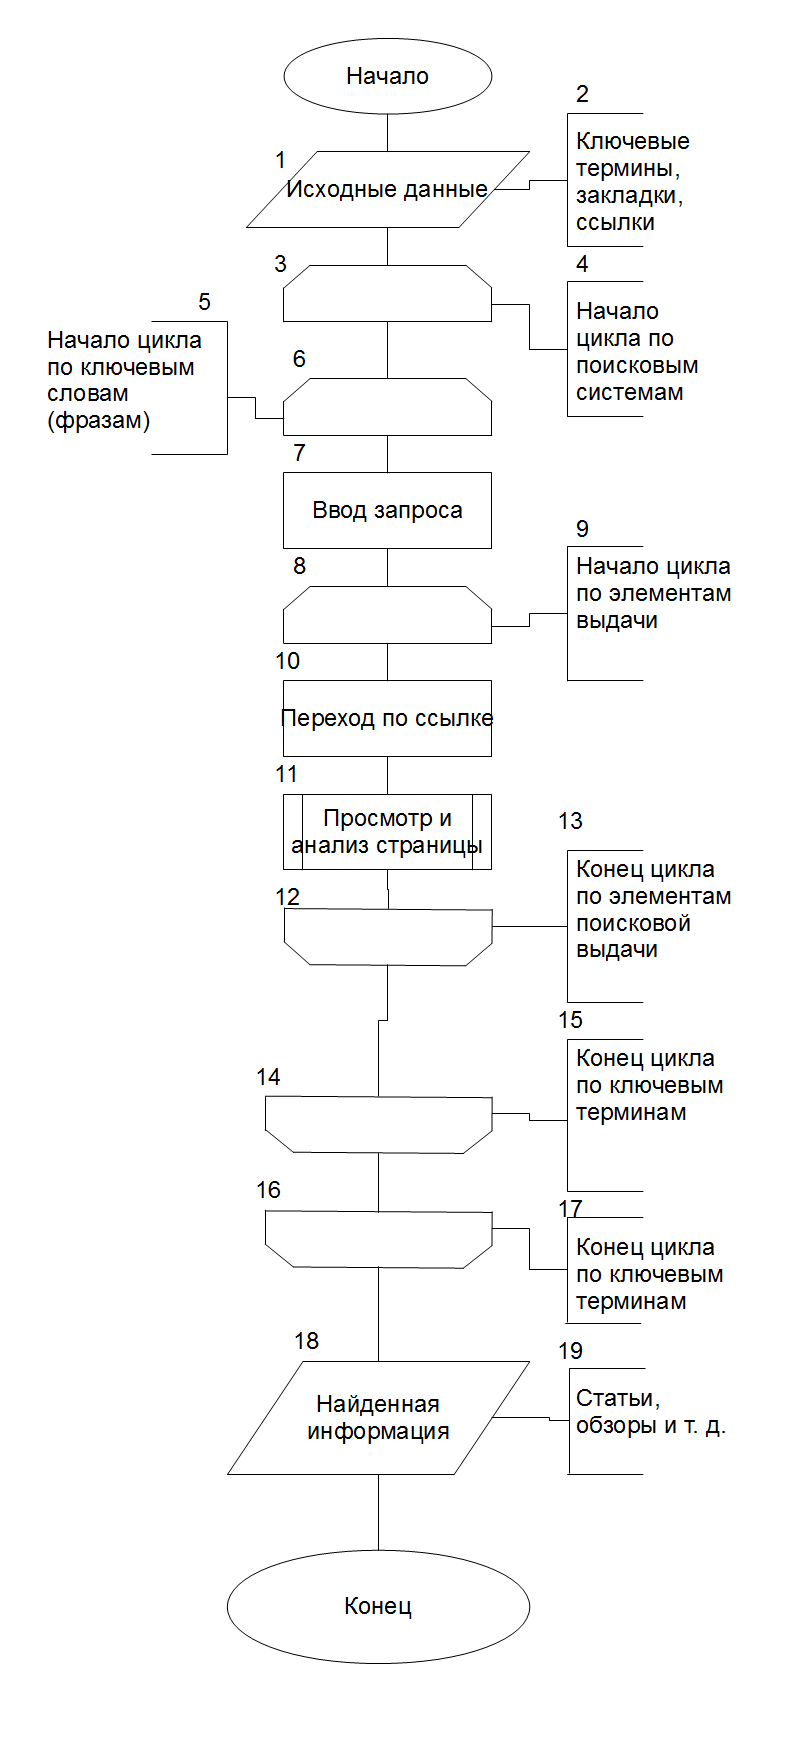
\includegraphics[scale=1.0]{images/searchalg.png}
	\caption{\small Алгоритм поиска информации в Интернете}
	\label{fig:searchalg}
\end{figure}

В приведённом на рисунке \ref{fig:searchalg} алгоритме использовались поисковые машины Google \cite{google}, Bing \cite{bing} и реже Yandex \cite{yandex}.

\subsubsection{Формирование требований к синтаксическому парсеру}
Выделение аналогов среди найденного производилось на основании максимального соответствия следующим предъявляемым к синтаксическим парсерам требованиям:
\begin{list}{\labelitemi}{\leftmargin=1.5cm}
	\item синтаксический парсер должен быть точным (минимальное число ошибок в результирующем дереве разбора, максимально корректное разрешение грамматически неоднозначных ситуаций) --- A;
	\item алгоритм синтаксического анализа должен быть эффективен (минимальная временная сложность алгоритма и сложность алгоритма по памяти, минимальное потребление памяти и процессорной мощности, максимальный потенциально возможный объём анализируемого текста) --- S;
	\item рассматриваемый аналог должен быть совместим с русским языком (минимальная степень специфичности грамматики по отношению к используемому языку, возможность реализовать формальную грамматику для русского языка на основе уже используемой парсером или наличие готовой) --- LS;
	\item входная информация должна быть в минимальной степени формализована (рассматриваемый аналог не должен требовать от входной информации предварительной обработки иными средствами естественноязыкового анализа) --- V.
\end{list}

\subsubsection{Критерии оценки аналогов}
Приведённые выше требования положены в основу четырёх критериев кортежной модели сравнения и оценки аналогов:\\
O = <A, S, LS, V; R>\\
где O --- интегральная оценка аналога, A --- критерий точности разбора, S --- критерий эффективности алгоритма, LS --- критерий простоты локализации грамматики, V --- критерий степени формализации входной информации, R --- матрица связи.

Методы оценки по выделенным критериям следующие:
\begin{list}{\labelitemi}{\leftmargin=1.5cm}
	\item A --- объективная нормированная процентная шкала, за нуль отсчёта взят минимальный показатель;
	\item S --- дискретная шкала, чем выше график производной функции сложности алгоритма, тем ниже оценка;
	\item LS --- дискретная шкала: 0.0 --- локализация грамматики невозможна, 0.25 --- для локализации необходима полная переработка грамматики, 0.50 --- достаточно изменить правила грамматики и провести машинное обучение, 0.75 --- достаточно отредактировать правила грамматики, 1.0 --- существует полноценная формальная грамматика русского языка;
	\item V --- дискретная шкала: 0.0 --- информация в виде метаданных, 0.50 --- информация в виде предварительно размеченного текста, 1.0 --- информация в виде необработанного текста.
\end{list}

Формула расчёта оценки аналога:

O \(= \alpha(A)*A + \alpha(S)*S + \alpha(LS)*LS + \alpha(V)*V\)\\
где 
\(\sum_{i=1}^{n} \alpha_i = 1\), \(\alpha_i\) --- весовой коэффициент соответствующего критерия, n --- количество критериев.

Найдём весовые коэффициенты методом попарного сравнения критериев Томаса Саати \cite{tsaati}. 
Будем использовать шкалу от 1 до 9, где: 
\begin{list}{\labelitemi}{\leftmargin=1.5cm}
  \item 1 --- равенство;
  \item 2 --- промежуточное значение;
  \item 3 --- слабое превосходство;
  \item 4 --- промежуточное значение;
  \item 5 --- сильное превосходство;
  \item 6 --- промежуточное значение;
  \item 7 --- значительное превосходство;
  \item 8 --- промежуточное значение;
  \item 9 --- абсолютное превосходство.
\end{list}
Матрица попарного сравнение представлена в таблице \ref{tab:crit}.

\begin{table}[H]
\centering
\caption{Матрица попарного сравнения критериев}
{\small 
\begin{tabu}to \textwidth{ | X[c] | X[c] | X[c] | X[c] | X[c] | X[c] | X[c] | }
	\hline
          & A   & S   & LS  & V & Среднее & Вес  \\ \hline
	A     & 1   & 3   & 4   & 7 & 3.75    & 0.51 \\
	S     & 1/3 & 1   & 3   & 5 & 2.33    & 0.31 \\
	LS    & 1/4 & 1/3 & 1   & 2 & 0.90    & 0.12 \\
	V     & 1/7 & 1/5 & 1/2 & 1 & 0.43    & 0.06 \\ \hline
	Сумма &     &     &     &   & 7.41    & 1.00 \\
	\hline
\end{tabu}
}
\label{tab:crit}
\end{table}

\subsubsection{Обзор найденных аналогов}

\subsubsection{Выбор прототипа}
Выделенные в требованиях характеристики для найденных аналогов были определены и сведены в таблице \ref{tab:obj}.

\begin{table}[H]
\centering
\caption{Результат объективной оценки аналогов по критериям}
{\small 
\begin{tabu}to \textwidth{ | X[c] | X[c] | X[c] | X[c] | X[c] | }
	\hline
    Аналог/Критерий & A    & S                & LS   & V   \\ \hline
	BLA                      & 75.9 & \(O(n^3)\)       & 0.50 & 1.0 \\ \hline
	SP                       & 72.8 & \(O(n^3*|G|^2)\) & 0.50 & 1.0 \\ \hline
	RG                       & 78.1 & \(O(n^5)\)       & 0.50 & 1.0 \\ \hline
	CYK                      & 66.6 & \(O(n^3*|G|)\)   & 0.75 & 0.5 \\ \hline
	IOA                      & 56.0 & \(O(n^3)\)       & 0.50 & 1.0 \\ \hline
	EA                       & 78.0 & \(O(n^3)\)       & 0.75 & 0.5 \\ \hline
	LGP                      & 73.0 & \(O(n^3)\)       & 1.00 & 1.0 \\ 
	\hline
\end{tabu}
}
\label{tab:obj}
\end{table}

С учётом приведённой ранее системы выставления оценок, объективные показатели были переведены в значения на соответствющих шкалах и нормированы. Результат представлен в таблице \ref{tab:scales}.

\begin{table}[H]
\centering
\caption{Результат нормированной оценки аналогов по шкалам критериев}
{\small 
\begin{tabu}to \textwidth{ | X[c] | X[c] | X[c] | X[c] | X[c] | }
	\hline
    Аналог/Критерий          & A    & S     & LS   & V   \\ \hline
	BLA                      & 0.97 & 1.00  & 0.50 & 1.0 \\ \hline
	SP                       & 0.93 & 0.50  & 0.50 & 1.0 \\ \hline
	RG                       & 1.00 & 0.00  & 0.50 & 1.0 \\ \hline
	CYK                      & 0.85 & 0.75  & 0.75 & 0.5 \\ \hline
	IOA                      & 0.72 & 1.00  & 0.50 & 1.0 \\ \hline
	EA                       & 1.00 & 1.00  & 0.75 & 0.5 \\ \hline
	LGP                      & 0.93 & 1.00  & 1.00 & 1.0 \\ 
	\hline
\end{tabu}
}
\label{tab:scales}
\end{table}

Взвешенные оценки, полученные умножением оценки по шкале на соответствующий весовой коэффициент, приведены в таблице \ref{tab:weight}.

\begin{table}[H]
\centering
\caption{Результат оценки аналогов по шкалам критериев}
{\small 
\begin{tabu}to \textwidth{ | X[c] | X[c] | X[c] | X[c] | X[c] | X[c] | }
	\hline
    Аналог/Крит.             & A    & S     & LS   & V    & Сумма \\ \hline
	BLA                      & 0.49 & 0.31  & 0.06 & 0.06 & 0.92  \\ \hline
	SP                       & 0.47 & 0.16  & 0.06 & 0.06 & 0.75  \\ \hline
	RG                       & 0.51 & 0.00  & 0.06 & 0.06 & 0.63  \\ \hline
	CYK                      & 0.43 & 0.23  & 0.09 & 0.03 & 0.78  \\ \hline
	IOA                      & 0.37 & 0.31  & 0.06 & 0.06 & 0.80  \\ \hline
	EA                       & 0.51 & 0.31  & 0.09 & 0.03 & 0.94  \\ \hline
	LGP                      & 0.47 & 0.31  & 0.12 & 0.06 & 0.96  \\ 
	\hline
\end{tabu}
}
\label{tab:weight}
\end{table}

\subsection{Критика прототипа}\newpage
  \indent \section{Моделирование модуля взаимодействия парсера русского языка с внешними базами знаний}

Моделирование --- исследование объектов познания на их моделях; построение и изучение моделей реально существующих объектов, процессов или явлений с целью получения объяснений этих явлений, а также для предсказания явлений, интересующих исследователя \cite{wiki_modelling}.

Модель --- система, исследование которой служит средством для получения информации о другой системе \cite{uemov}.

В этой главе представлен результат работы по моделированию модуля взаимодействия парсера русского языка и внешних БЗ (онтологий) в виде следующих видов моделей: концептуальные, информационные, структурные, функционально-структурные и алгоритмические. Локальной целью является получение пакета моделей, достаточного для начала проектирования модуля.

\subsection{Концептуальные модели}

Концептуальная (содержательная) модель --- это абстрактная модель, определяющая структуру моделируемой системы, свойства её элементов и причинно-следственные связи, присущие системе и существенные для достижения цели моделирования.

Для описания концептуальной модели используется фреймовый формализм, а именно описание концептуальной модели в соответствии с ролевым фреймом \cite{gold}.

Концепция = <Ф, П, С, Н, Ц>, где Ф --- основные функции системы, П --- путь реализации основных функций системы, С --- структурная основа системы, Н --- направленность функционирования, Ц --- цель функционирования.

\subsubsection{Общие концептуальные модели}

Для начала приведём общие концептуальные модели частей внешней среды, принимающих участие во взаимодействии посредством моделируемого модуля.

\textbf{Парсер} --- программный продукт, модуль или библиотека, функцией которого является синтаксический анализ входных последовательностей строк на естественном или формальном искусственном языке путём генерации дерева разбора, определения его принадлежности к языку и корректировки на основе формальной грамматики языка и алгоритма парсинга, направленный на дальнейшую автоматическую или автоматизированную обработку результата с целью извлечения знания.

\textbf{База знаний} --- информационная структура, база данных, функцией которой является хранение и оперирование знаниями (метаданными) о некоторой области знания посредством структурирования исходных фактов и логического вывода новых на основе правил продукции и принципов построения баз знаний, направленных на предоставление максимально полной информации с целью поддержки деятельности пользователя.

\textbf{Онтология} --- форма представления знаний, выполняющая функцию хранения детального описания некоторой области знания посредством структурирования классов объектов, связей между ними, их атрибутов и ограничений на основе спецификаций Semantic Web и языка OWL, направленных на формализацию предметной области с целью поддержки деятельности пользователя.

\subsubsection{Базово-уровневая концептуальная модель}

\textbf{Интерфейс онтология-парсер} --- программный модуль или библиотека, функциями которого являются организация доступа парсера к внешнему хранилищу знаний в виде онтологии, отправка запросов, трансляция в формат парсера и кэширование полученных ответов, передача парсеру необходимых правил продукции посредством получения исходного слова через прикладной программный интерфейс, генерации SPARQL-запроса по полученному слову, отправки запроса, разбору и временному хранению результата для передачи в алгоритм, на основе протоколов взаимодействия с семантичечкими хранилищами и спецификаций прикладного программного интерфейса парсера, направленный на увеличение релевантности, актуальности и корректности используемой парсером синтаксической информации с целью повышения качества обработки и снижения накладных расходов на модернизацию и/или новую разработку.

\subsection{Информационная модель модуля взаимодействия онтология-парсер}

Приведённая на рисунках \ref{fig:infomodel0} --- \ref{fig:infomodel3} информационная модель отображает иерархическое распределение информации по уровням её абстракции по мере декомпозиции структурных единиц моделируемого модуля.

\begin{figure}[H]
	\centering
		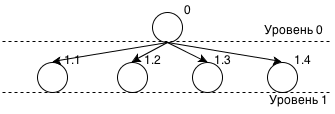
\includegraphics[scale=1.0]{images/infomodel0.png}
	\caption{\small Информационная модель, уровни 0 и 1}
	\label{fig:infomodel0}
\end{figure}

Обозначения на рисунке \ref{fig:infomodel0}: 0 --- рабочая информация модуля, 1.1 --- данные парсера, 1.2 --- информация в кэше, 1.3 --- внутренние данные генератора запросов, 1.4 --- данные онтологии.

\begin{figure}[H]
	\centering
		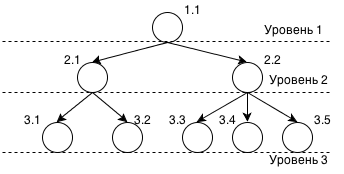
\includegraphics[scale=1.0]{images/infomodel1.png}
	\caption{\small Декомпозиция узла 1.1}
	\label{fig:infomodel1}
\end{figure}

Обозначения на рисунке \ref{fig:infomodel1}: 1.1 --- данные парсера, 2.1 --- исходные данные, 2.2 --- синтаксическая информация, 3.1 --- входная последовательность, 3.2 --- метаданные, 3.3 --- синтаксические структуры, 3.4 --- морфологические метки, 3.5 --- связи.

\begin{figure}[H]
	\centering
		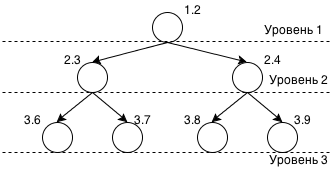
\includegraphics[scale=1.0]{images/infomodel2.png}
	\caption{\small Декомпозиция узла 1.2}
	\label{fig:infomodel2}
\end{figure}

Обозначения на рисунке \ref{fig:infomodel2}: 1.2 --- данные кэша, 2.3 --- ключи, 2.4 --- значения, 3.6 --- слова, 3.7 --- метки, 3.8 --- правила, 3.9 --- элементы запросов.

\begin{figure}[H]
	\centering
		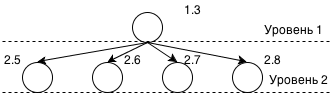
\includegraphics[scale=1.0]{images/infomodel3.png}
	\caption{\small Декомпозиция узла 1.3}
	\label{fig:infomodel3}
\end{figure}

Обозначения на рисунке \ref{fig:infomodel3}: 1.3 --- данные генератора/транслятора, 2.5 --- ключевые слова, 2.6 --- макеты запросов, 2.7 --- правила генерации запросов, 2.8 --- реквизиты доступа к внешней БЗ.

\subsection{Системно-структурная модель парсера русского языка}

Системно-структурные модели представляют моделируюмую систему в виде структурных блоков, связанных информационными либо материальными связями (путями прохождения информации).

На основе критики прототипа, приведённой в главе 1, и его структурной модели (рисунок \ref{fig:prototype_struct}), сформируем новую структурную модель, в которой учтём предложение по усовершенствованию прототипа. Модель представлена на рисунке \ref{fig:modifiedstruct}.

\begin{figure}[H]
	\centering
		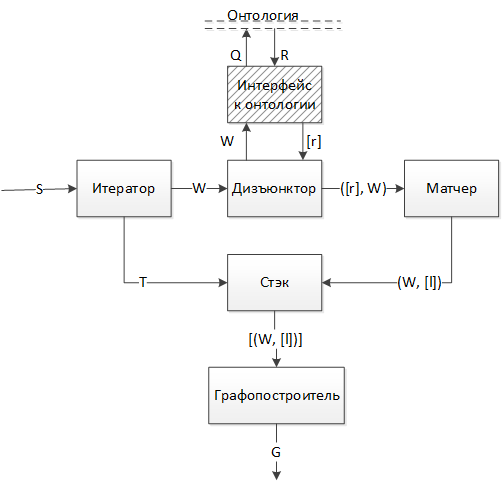
\includegraphics[scale=1.0]{images/modifiedstructure.png}
	\caption{\small Структурная модель модифицированного прототипа}
	\label{fig:modifiedstruct}
\end{figure}

На рисунке \ref{fig:modifiedstruct} добавляемый блок (Интерфейс к онтологии), замещающий собой блок прототипа Словарь, помечен штриховкой. Новые обозначения: Q --- SPARQL-запрос к онтологии, R --- ответ онтологии по запросу Q.

Декомпозиция блока Интерфейс к онтологии приведена на рисунке \ref{fig:decomposedstruct}.

\begin{figure}[H]
	\centering
		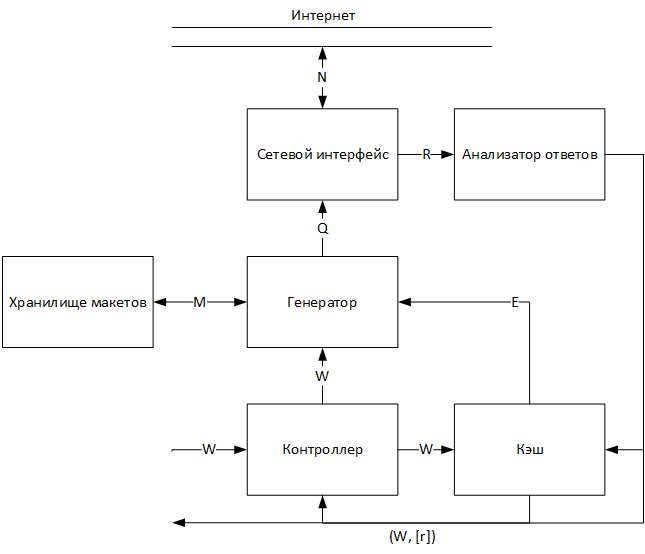
\includegraphics[scale=1.0]{images/decomposedstructure.png}
	\caption{\small Декомпозиция модуля Интерфейс к онтологии}
	\label{fig:decomposedstruct}
\end{figure}

Блок Контроллер принимает на вход слово W и выступает в роли ядра модуля, организующего связь между структурными элементами. Слово W передаётся в Кэш, откуда, если найдены, возвращаются правила для данного слова ([r]); в противном случае слово W передаётся Контроллером в Генератор запросов, использующий макеты (M) Хранилища макетов и кэшированные элементы E для генерации SPARQL-запроса Q, передаваемого в Сетевой интерфейс. Сетевой интерфейс взаимодействует с онтологией посредством двунаправленного потока сетевых пакетов (N), полученные данные (R) передаются в Анализатор ответов, преобразующий их в правила грамматики связей. Результат сохраняется в Кэш и передаётся в  Контроллер, возвращающий данные парсеру.

\subsection{Алгоритмическая модель}

Алгоритмическая модель изображает процесс работы алгоритма модуля при помощи блоков-подпроцессов и связей управления между ними. На рисунках \ref{fig:initialalgorithmA} и \ref{fig:initialalgorithmB} изображён алгоритм работы исходного парсера (прототипа без модификаций).

\begin{figure}[H]
	\centering
		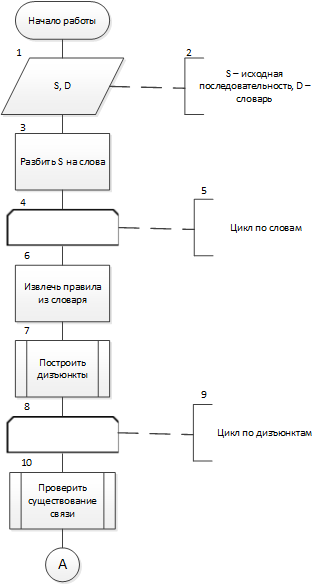
\includegraphics[scale=1.0]{images/initialalgorithmA.png}
	\caption{\small Алгоритм работы прототипа (начало)}
	\label{fig:initialalgorithmA}
\end{figure}

\begin{figure}[H]
	\centering
		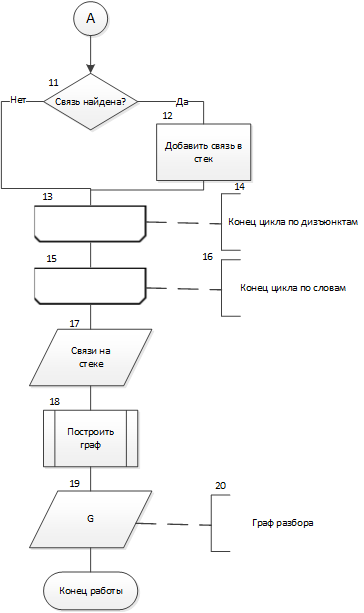
\includegraphics[scale=1.0]{images/initialalgorithmB.png}
	\caption{\small Алгоритм работы прототипа (окончание)}
	\label{fig:initialalgorithmB}
\end{figure}

Модифицированный алгоритм представлен на рисунках \ref{fig:modifiedalgorithmA} и \ref{fig:modifiedalgorithmB}, добавленные процессы помечены штриховкой, блоки 6 и 7 в сумме соответствуют блоку <<Интерфейс к онтологии>> структурной модели модифицированного прототипа (рисунок \ref{fig:modifiedstruct}.

\begin{figure}[H]
	\centering
		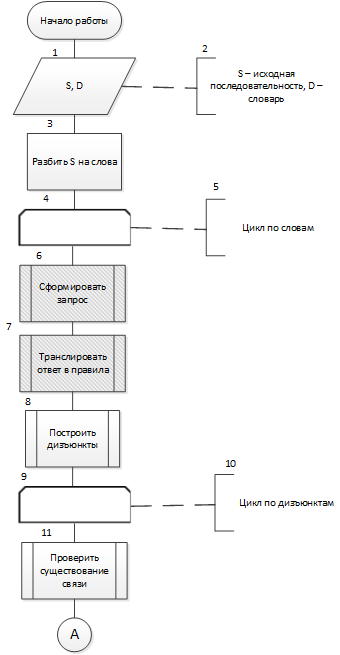
\includegraphics[scale=1.0]{images/modifiedalgorithmA.png}
	\caption{\small Алгоритм работы парсера с учётом предлагаемого решения (начало)}
	\label{fig:modifiedalgorithmA}
\end{figure}

\begin{figure}[H]
	\centering
		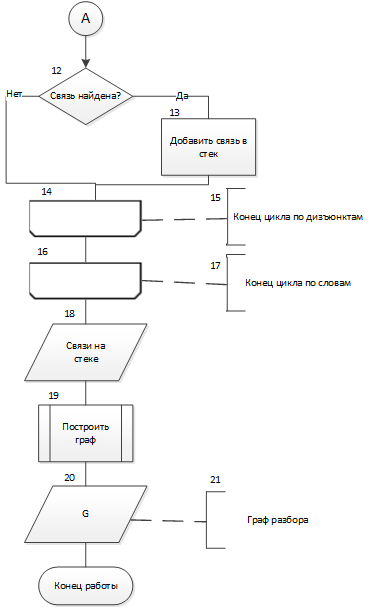
\includegraphics[scale=1.0]{images/modifiedalgorithmB.png}
	\caption{\small Алгоритм работы парсера с учётом предлагаемого решения (окончание)}
	\label{fig:modifiedalgorithmB}
\end{figure}

Декомпозиция блока 6 дана на рисунке \ref{fig:decomposedalgorithm1}.

\begin{figure}[H]
	\centering
		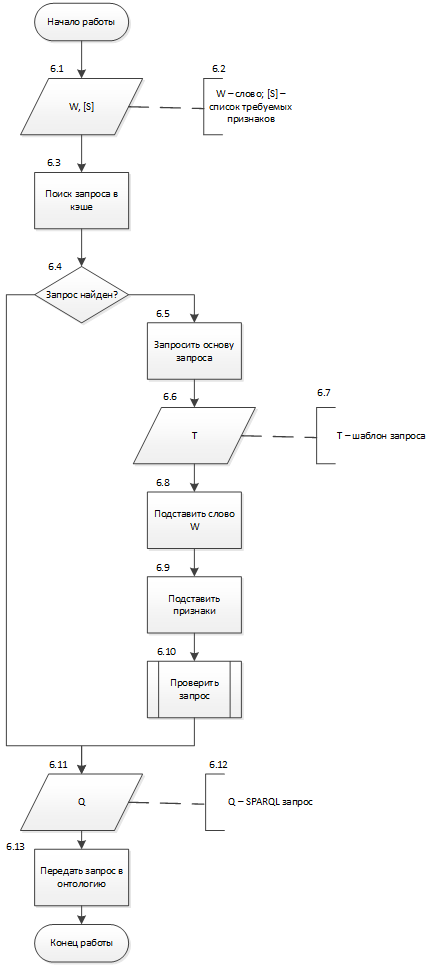
\includegraphics[scale=0.95]{images/decomposedalgorithm1.png}
	\caption{\small Декомпозиция блока 6}
	\label{fig:decomposedalgorithm1}
\end{figure}

Декомпозиция блока 7 приведена на рисунке \ref{fig:decomposedalgorithm2}.

\begin{figure}[H]
	\centering
		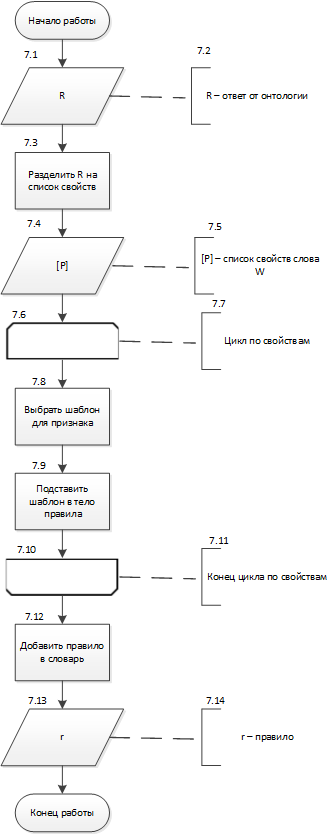
\includegraphics[scale=1.0]{images/decomposedalgorithm2.png}
	\caption{\small Декомпозиция блока 7}
	\label{fig:decomposedalgorithm2}
\end{figure}

\subsection{Результаты и выводы по главе 2}

В процессе моделирования прототипа были достигнуты следующие результаты:
\begin{list}{\labelitemi}{\leftmargin=1.5cm}
	\item получены концептуальные модели сущностей, участвующих в работе прототипа;
	\item построена иерархия информации внутри модифицированного прототипа;
	\item получены структурные модели модифицированного прототипа и добавляемого блока;
	\item получены алгоритмические модели работы исходного и модифицируемого прототипа, а также алгоритмы работы добавляемого блока.
\end{list}

\textbf{Вывод}: в результате моделирования получено новое знание в виде пакета моделей. Полученной информации достаточно для перехода к стадии проектирования предлагаемого решения.
\newpage
  \indent \section{Проектирование модуля взаимодействия парсера русского языка с внешней онтологией}

В данной главе  рассмотрено внешнее и внутреннее проектирование. Внешнее проектирование --- этап проектирования объекта как сложной иерархической системы, состоящий в рассмотрении его как части системы более высокого уровня. Результатом такого проектирования является исходный вариант технического задания, которое может уточняться и корректироваться в процессе внутреннего проектирования объекта. Внутреннее проектирование - этап проектирования объекта как сложной иерархической системы, выполняемый на основании внешнего проектирования и состоящий в рассмотрении его как самостоятельной системы.

\subsection{Внешнее проектирование}

\subsubsection{Целеполагание}

Задача системы --- взять на себя взаимодействие с хранилищами синтаксической информации, заменив локальные словари парсеров, таким образом достигнув \textbf{глобальную цель} --- повышение качества используемых парсерами данных о синтаксисе ЕЯ.

Глобальную цель можно представить в виде композиции следующих локальных целей:

\begin{list}{\labelitemi}{\leftmargin=1.5cm}
	\item обеспечить взаимодействие синтаксического парсера с модулем на уровне API;
	\item обеспечить генерацию SPARQL-запросов из получаемых парсером слов;
	\item обеспечить сетевое взаимодействие с внешним хранилищем синтаксических знаний (OWL, RDF Scheme);
	\item обеспечить преобразование полученного в формате онтологии ответа в правила парсера и передачу их в парсер для продолжения обработки текста.
\end{list}

Достижение вышеупомянутых целей позволит снять с разработчика парсера ответственность за разработку и поддержание грамматики парсера, позволит использовать в работе парсера наиболее полный и корректный источник знаний, упростит разработку и развитие парсера.

\subsubsection{Выработка требований к системе}

Поскольку модуль взаимодействия парсера русского языка с онтологией (далее Модуль) представляет собой интерфейс, наиболее критичным при проектировании являются протоколы и способы обмена информацией в точках соприкосновения Модуля с соединяемыми элементами надсистемы.

При внешнем проектировании в данной работе в качестве экземпляра парсера используется реализация парсера грамматики связей от AbiWord \cite{abiparser}. По состоянию на май 2013, он находится в версии 4.7 и предоставляет готовую грамматику для русского языка, которую можно использовать в качестве образца для генерации правил и для контроля корректности работы Модуля.

Упомянутый парсер предоставляет API \cite{api}, с помощью которого разумно реализовать взаимодействие с Модулем. Такая реализация значительно увеличит производительность результирующего решения за счёт отсутствия каналов передачи информации между парсером и Модулем и нивелирования накладных расходов на двустороннее преобразование типов данных в точке соприкосновения. С другой стороны, реализация на основе API неизбежно накладывает ограничения на язык программирования: у выбранной технологиии должна быть возможность реализовать бинарный интерфейс с программами, написанными на C.

Со стороны онтологии Модуль должен использовать технологию, предоставляемую стэком Semantic Web \ref{fig:swstack}. Жёлтым цветом на рисунке выделены протоколы, используемые для взаимодействия с семантическими хранилищами извне (язык запросов SPARQL и формат описания RDF). 

\begin{figure}[H]
	\centering
		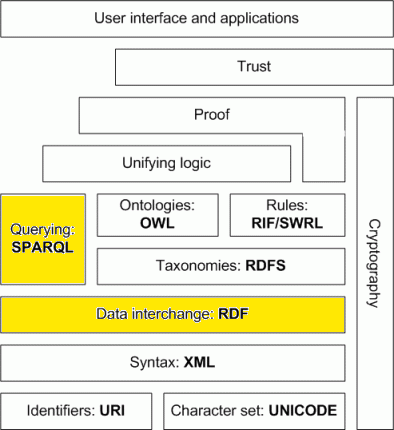
\includegraphics[scale=1.0]{images/swstack.png}
	\caption{\small Стэк технологий SW}
	\label{fig:swstack}
\end{figure} 

Таким образом, со стороны семантического хранилища Модуль должен реализовывать обмен данными посредством сетевого протокола HTTP, отправляемые данные имеют формат запроса SPARQL, принимаемые --- RDF (XML). Полученный от хранилища XML необходимо десериализовать (преобразовать во внутренний формат данных) и передать парсеру извлечённые из него данные.

В демонстрационных целях, в качестве хранилища будет использовать самостоятельно созданная OWL-онтология.

Поскольку проектируемый Модуль базируется на разработке AbiWord, являющейся открытым проектом и распространяющейся под лицензией GPL \cite{gpl}, код Модуля также обязан подчиняться правилам лицензии, быть открытым и свободно распространяемым. 

\subsubsection{Выработка требований к функционированию}

Второй ключевой характеристикой функционирования является скорость одной итерации от получения слова до возвращения правил парсеру. Синтаксическая информация изменяется крайне редко (в основном, в случае корректировок и дополнений), поэтому вероятность изменения полученных правил за время их оборота в системе пренебрежимо мала. С этой точки зрения, разумно обязать Модуль кэшировать информацию по уже обработанным словам, чтобы избежать повторного цикла.

Необходимость использования Модуля в виде отдельного приложения отсутствует, основная работа по анализу текстовых последовательностей выполняется в парсере. Таким образом, разумно оформить Модуль в виде разделяемой библиотеки, подключаемой парсером в процессе запуска.

API Link Parser'а не предоставляет возможностей получения конфигурации, переданной собственно парсеру, таким образом, необходимо обеспечить возможность конфигурировать библиотеку отдельно. Создание отдельного интерфейса конфигурации нецелесообразно в связи с небольшим числом настроек, следовательно, достаточно предусмотреть чтение библиотекой конфигурации из файла.

Проектируемый Модуль использует API Link Parser'a, однако технология не ограничивается отдельной реализацией и даже отдельным методом парсинга. Подобный интерфейс возможно применить к любому парсеру, основанному на контекстно-свободных грамматиках. С этой точки зрения, во время внутреннего проектирования необходимо предусмотреть возможность замены подсистемы, отвечающей за связь с парсером, без модификации остальных подсистем Модуля.

\subsubsection{Выработка требований к совместимости}

Проектируемый Модуль в конечном итоге является разделяемой библиотекой, используемой парсером. Таким образом, он не может предъявлять больше требований к нижележащей платформе, чем собственно парсер. В случае с Link Parser'ом, это любая Linux-подобная операционная система, обладающая необходимым для сборки парсера набором библиотек. Следует также предусмотреть кроссплатформенность, то есть, при внутреннем проектировании нельзя допускать использование компонентов, функционирование которых на платформах, отличных от текущей, невозможно или ограничено по каким-либо причинам.

\subsubsection{Выработка требований к показателям назначения}

Как уже было сказано, одним из ключевых показателей является скорость выполнения одной итерации по слову. С учётом сетевых задержек, скорость обработки одного слова не должна превышать одной секунды. В худшем случае, такая задержка обеспечит разбор фразы из двух-трёх десятков слов менее, чем за минуту.

В случае сетевой недоступности онтологии, отсутствия в ней слова либо сбоя внутри Модуля нельзя прерывать функционирование системы в целом. Логично предусмотреть обработку подобных исключительных ситуаций с переходом в <<безопасный режим>>, в котором парсер продолжает работу, используя в качестве источника информации внутренние словари.

\subsubsection{Выработка требований к видам обеспечения}

\textbf{Информационное обеспечение}

Хранимую в модуле информацию можно разделить на две части: макеты SPARQL-запросов и локальный кэш. 

Макеты целесообразно хранить в виде констант кода Модуля либо во внешних файлах в сериализованном виде и загружать при первом запросе к Модулю. Их объём мал, не требуется возможности их модификации, удаления или добавления.

Локальный кэш хранит правила для уже обработанных слов, элементы запросов и различную вспомогательную информацию. Нецелесообразно использовать для хранения подобных слабо структурированных данных реляционные БД. Возможно использование документ-ориентированных БД либо хранилищ типа <<ключ-значение>> (KVS). Информация в документ-ориентированных БД может храниться длительное время, перезагрузка СУБД не повлияет на неё. Однако, KVS значительно производительнее, и, с учётом того, что потеря информации из кэша не критична для функционирования системы в целом, предлагается использовать именно их. Также необходимо предусмотреть возможность работы без кэша, поскольку собственно парсер не требует наличия KVS в операционной системе.

\textbf{Используемые языки высокого уровня}

Исходный парсер реализован с помощью языка программирования С. Однако, его API не ограничивает нас использованием единственного языка. На практике реализация Модуля возможна на любом языке высокого уровня с доступным FFI (интерфейсом внешних функций). В данной работе в качестве основного языка программирования был выбран Haskell \cite{haskell}, сильными сторонами которого являются типизация, сильно сокрающая объём работ по отладке, перенося их на стадию внутреннего проектирования, минимальный объём кода, необходимый для получения работоспособного приложения и наличие различных библиотеку, способных упростить разработку. Также Haskell является компилируемым языком, не использует виртуальные машины и интерпретаторы, что положительно сказывается на производительности. Реализации Haskell доступны для большинства современных операционных систем.

\textbf{Программное обеспечение}

Сборка исходного парсера требует компилятора языка C (gcc, Intel C Compiler), программ make и autoconfig. В операционных системах Windows данные программы отсутствуют, поэтому может возникнуть необходимость использовать порты MinGW либо CYGWIN.

Сборка Модуля, помимо того, требует наличия компилятора Haskell (Glasgow Haskell Compiler либо HUGS), пакетная система cabal. Под Windows рекомендуется использовать пакет Haskell Platform.

В качестве кэша рекомендуется использовать Memcached либо Redis. Redis предпочтительнее из-за своей перзистентности, то есть, его перезагрузка не приведёт к потере кэшированной информации.

\subsection{Внутреннее проектирование}

На основании требований, выделенных выше, мы можем уточнить структуру проектируемого Модуля, типизировав потоки информации и выделив ключевые функции в исходном коде Модуля.

\subsubsection{Ключевые функции}

Для замены словаря на интерфейс, предоставляемый Модулем, необходимо в API выделить ключевые функции, использующие словарь, и заменить либо исключить их.

Для описания функций будет использоваться Haskell-нотация (имя функции :: (ограничения классов типов) \(\Rightarrow\) тип1 \(\rightarrow\) тип2 \(\rightarrow\) тип3 \(\rightarrow\) \textellipsis \(\rightarrow\) типN).

Согласно \cite{api}, работа парсера начинается с создания словаря для языка, переданного в парсер из стандартного ввода (dictionary_create_language :: Строка -> Словарь). Возвращаемый функцией словарь нигде не будет использован, поэтому функция может быть исключена.

Следующая ключевая функция, в которой используется словарь, --- sentence_create :: Строка \(\rightarrow\) Словарь \(\rightarrow\) Размеченная последовательность. Её задача --- разметить входную последовательность слов в соответствии с переданным словарём. Достаточно будет переопределить эту функцию, сохранив её сигнатуру, но игнорируя словарь, вызывать нижележащие функции и процедуры, организующие взаимодействие с онтологией.

На стороне интерфейса с онтологией две ключевые функции, отвечающие за взаимодействие Модуля с хранилищем --- generateQuery :: Строка \(\rightarrow\) SPARQL и extractRules :: RDF \(\rightarrow\) Строка. Они условно соответствуют блокам 6 и 7 в алгоритмической модели модифицированного прототипа (рисунок \ref{fig:modifiedalgorithmA}).

Учитывая выше сказанное, приведём уточнённую и типизированную структурную модель проектируемого Модуля (рисунок \ref{fig:typedstructure}).

\begin{figure}[H]
	\centering
		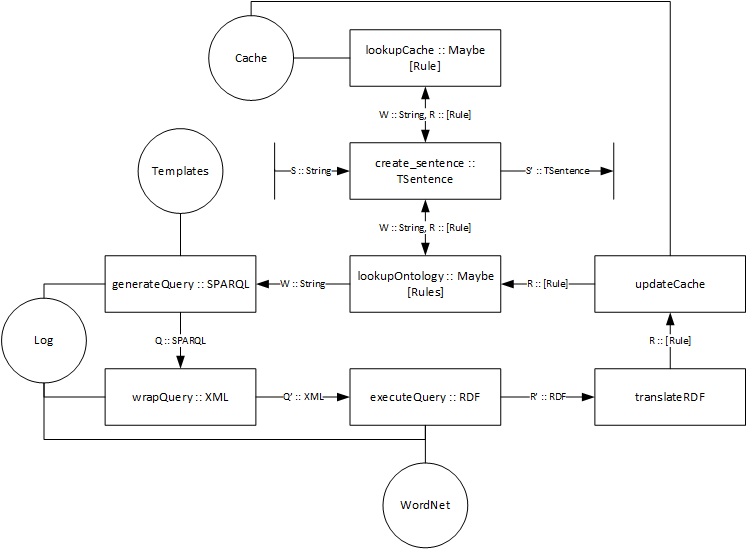
\includegraphics[scale=0.8]{images/typedstructure.png}
	\caption{\small Уточнённая структурная модель Модуля}
	\label{fig:typedstructure}
\end{figure} 

Приведённая модель опирается на принципы функционального программирования, то есть, разработку программ на основе их функциональной структуры и потоков данных, а не последовательности выполнения процедур (как в императивном программировании). Обозначения на рисунке \ref{fig:typedstructure}:

\begin{list}{\labelitemi}{\leftmargin=1.5cm}
	\item create_sentence --- точка входа, основная функция, принимающая на вход строку S и возвращающая размеченную строку S';
	\item lookupCache --- ищет в кэше правила по слову W, в соответствии с монадой Maybe, возвращает список правил R либо пустое значение;
	\item lookupOntology --- точка входа в подпроцесс поиска слова в онтологии, принимает на вход слово W, возвращает список правил R либо пустое значение;
	\item generateQuery --- с помощью хранилища шаблонов на основе слова W генерирует SPARQL-запрос Q, описывая все действия в журнале Модуля;
	\item wrapQuery --- оборачивает запрос Q в форму Q', пригодную для передачи по сети;
	\item executeQuery --- отсылает запрос Q' на сервер онтологии, дожидается ответа, пишет результат в журнал;
	\item translateRDF --- транслирует полученный RDF-ответ R' в список правил (возможно, пустой) R;
	\item updateCache --- обновляет кэш, записывая туда соответствие списка правил R слову W, после чего завершает работу, возвращая полученный список в точку входа.
\end{list}

\subsection{Результаты и выводы по главе 3}

В процессе проектирования Модуля были достигнуты следующие результаты:
\begin{list}{\labelitemi}{\leftmargin=1.5cm}
	\item сформулированы требования к функционированию, структуре и платформе проектируемой системы;
	\item структура прототипа разложена на программные функции верхнего уровня, уточнена схемой движения информации и типизирована;
	\item выполнено системно обоснованное техническое задание на разработку модуля взаимодействия парсера русского языка с онтологией (приложение А).
\end{list}

\textbf{Вывод}: полученной в результате проектирования информации достаточно для перехода к стадии инженерной реализации проекта.\newpage
  \indent \section{Инженерная реализация модуля взаимодействия парсера русского языка с онтологией}

\subsection{Детали реализации}

Реализация предлагаемого решения производилась с использованием языка Haskell спецификации Haskell 2010 \cite{haskell2010}, добавляюшая в стандарт языка FFI, а также регламентирующей ряд синтаксических изменений. Для компиляции библиотеки использовался компилятор Glasgow Haskell Compiler (GHC) версии 7.4.2 под управлением XUbuntu Linux 12.10 (версия ядра 3.5.0, архитектура x86).

Для взаимодействия с парсером использовалось API Link Parser \cite{api}, для взаимодействия с онтологией были выбраны библиотеки hsparql, предоставляющая DSL для генерации SPRARQL-запросов, и rdf4h, описывающая типы данных RDF в нотации языка Haskell.

Для сетевого взаимодействия использовались методы, предоставляемые стандартной библиотекой GHC и Haskell Platform.

При разработке использовался текстовый редактор Sublime Text 2 и система управления версиями Git. Код библиотеки является открытым, распространяется свободно, и на момент написания диссертации был доступен по адресу \url{https://github.com/lumrandir/tomahawk}.

Для моделирования и описания демонстрационных онтологий использовалась система Protege.

Парсер был реализован в виде веб-приложения topor-web, поскольку это упрощало работу над пользовательским интерфейсом и позволяло обойти проблемы с демонстрацией под различными платформами.

\subsection{Руководство по развёртыванию и эксплуатации парсера русского языка Link Parser с библиотекой tomahawk}

\subsubsection{Предварительные замечания}

Для выполнения описанного в представленном руководстве процесса на компьютере пользователя должна быть установлена операционная система
Ubuntu (KUbuntu, XUbuntu, Linux Mint, Debian) либо иная операционная система, оснащённая пакетным менеджером apt. Рекомендуется использование Ubuntu 12.10.

Развёртывание парсера на компьютерах с другими Unix-системами с помощью данного руководства допустимо, однако, возможны отличия:
названия пакетов и используемые пакетные менеджеры и/или способы установки пакетов могут отличаться от представленных в руководстве, хотя
последовательность действий совпадает.

Развёртывание парсера на операционных системах Windows не является предметом рассмотрения данного руководства, поскольку связано с
дополнительными инфраструктурными сложностями, препятствующими достижению демонстрационной цели.

\subsubsection{Установка необходимых компонентов}

Поскольку topor-web представляет из себя веб-ориентированную
клиент-серверную систему, распространяющуюся в виде исходного кода, для
полноценного развёртывания нам понадобятся следующие компоненты:

\begin{list}{\labelitemi}{\leftmargin=1.5cm}
	\item nginx – проксирующий веб-сервер, задачей которого является
маршрутизация запросов из внешней сети в веб-приложение,
поддерживающее работу системы;
	\item redis – документ-ориентированное сетевое журналируемое хранилище
данных типа <<ключ-значение>>; используется в качестве кэширующего
хранилища возвращаемых из онтологии данных;
	\item ruby – интерпретатор языка программирования Ruby, с использованием
которого выполнена реализация веб-приложения;
	\item ghc – компилятор языка программирования Haskell, с использованием
которого выполнена реализация генератора запросов к онтологии tomahawk;
	\item gcc – компилятор языка программирования C, с использованием
которого реализовано ядро парсера Link Grammar;
	\item git – распределённая система контроля версий; использование этого
компонента опционально, получить исходный код можно в виде архива.
\end{list}

\subsubsection{Получение исходного кода системы}

Система topor-web распространяется в виде исходного кода. Это значит,
что пользователь системы должен самостоятельно собрать готовую систему.

Получить исходный код системы можно двумя способами:
\begin{list}{\labelitemi}{\leftmargin=1.5cm}
\item клонирование репозитария кода системы с помощью системы
контроля версий;
\item получение исходного кода в виде архива.
\end{list}

Для клонирования репозитария пользователь должен установить
систему контроля версий Git. В операционной системе Ubuntu установка Git
производится при помощи команды:

\begin{lstlisting}[language=bash]
sudo apt-get install git
\end{lstlisting}

После успешной установки системы Git пользователь должен перейти в
каталог, где будет располагаться система topor-web. Например, копия
репозитария может располагаться в домашней папке пользователя, переход в
котрую осуществляется командой:

\begin{lstlisting}[language=bash]
cd ~
\end{lstlisting}

Войдя в нужную директорию, пользователь должен выполнить
следующую команду:

\begin{lstlisting}[language=bash]
git clone git://github.com/lumrandir/topor-web.git
\end{lstlisting}

В результате выполнения этой команды пользователь получит наиболее
актуальный исходный код системы topor-web, который будет помещён внутрь
директории topor-web по текущему пути. То есть, полный путь к каталогу с
системой будет выглядеть как ~/topor-web. Этот каталог в дальнейшем будем
называть корневым каталогом приложения.

Второй способ заключается в следующем:

\begin{list}{\labelitemi}{\leftmargin=1.5cm}
\item получить архив исходного кода системы по следующей ссылке:
\url{https://github.com/lumrandir/topor-web/archive/master.zip};
\item распаковать полученный архив в нужную директорию.
\end{list}

Получение исходного кода выполняется командами:

\begin{lstlisting}[language=bash]
cd ~ && wget https://github.com/lumrandir/\
topor-web/archive/master.zip
unzip master.zip && mv topor-web\{-master,\}
\end{lstlisting}

После чего в каталоге topor-web внутри текущего также будет
располагаться актуальный исходный код системы.

\subsubsection{Установка интерпретатора языка программирования Ruby}

Для работы системы предпочтительно использовать стандартный
интерпретатор CRuby версии равной или выше 1.9.1.

Работа системы topor-web на альтернативных интерпретаторах (JRuby,
Rubinius, REE) не тестировалась и не гарантируется.

Установка CRuby в Ubuntu выполняется следующим образом:

\begin{lstlisting}[language=bash]
sudo apt-get install ruby
\end{lstlisting}

Вместе с пакетом ruby будет установлен менеджер библиотек Ruby gem.
Для работы системы потребуется установить библиотеку bundler:

\begin{lstlisting}[language=bash]
sudo gem install bundler
\end{lstlisting}

Bundler осуществляет контроль зависимостей, при запуске системы он
проверяет наличие необходимых ruby-библиотек. После установки bundler необходимо войти в корневой каталог
приложения и выполнить установку необходимых библиотек: 

\begin{lstlisting}[language=bash]
bundle install.
\end{lstlisting}

Проверить запуск системы можно с помощью команды: 

\begin{lstlisting}[language=bash]
bundle exec unicorn
\end{lstlisting}

Данная команда запустит многопоточный веб-сервер unicorn. Работу
приложения можно проверить, запустив веб-браузер и перейдя по адресу
\url{http://localhost:8080/version}. Пользователь должен увидеть текущую версию
приложения и статус библиотек парсера (в данном случае статус будет
<<Библиотеки недоступны>>).

\subsubsection{Установка компиляторов библиотек парсера}

Для сборки библиотек Link Grammar парсера пользователю потребуются
компиляторы gcc и ghc, также система контроля версий subversion.
Последовательность команд для сборки библиотеки парсера следующая
(выполняется в корневом каталоге приложения):

\begin{lstlisting}[language=bash]
sudo apt-get install subversion
svn co http://svn.abisource.com/link-grammar/trunk
link-grammar
cd link-grammar
sudo apt-get install make gcc automake libtool ant
./autogen.sh
./configure
make
sudo make install
sudo ldconfig
\end{lstlisting}

Приведённая последовательность действий устанавливает пакеты make
(система автоматизированной компиляции), gcc (GNU Compiler Collection ---
компилятор языка Си), automake и libtool --- генераторы конфигурационных
файлов компиляции. После установки пакетов осуществляется конфигурация
(создание сценариев компиляции с учётом текущего состояния системы) и
собственно сборка парсера. Последние два шага устанавливают собранные
библиотеки в системные каталоги и осуществляют их регистрацию.

Следующий шаг --- сборка модуля взаимодействия с онтологией:

\begin{lstlisting}[language=bash]
cd ../tomahawk
sudo apt-get install ghc cabal-install
make
\end{lstlisting}

Эта последовательность действий устанавливает компилятор ghc
(Glasgow Haskell Compiler) и пакетный менеджер cabal (аналог rubygems для
инфраструктуры языка Haskell).

Выполнив описанные выше шаги, пользователь может вновь запустить
сервер системы командой bundle exec unicorn из корневой папки
приложения и перейти на страницу \url{http://localhost:8080/version} в веб-браузере.
В случае корректной сборки и установки библиотек их статус изменится на
<<Доступны>>.

\subsubsection{Установка хранилища Redis}

Установка redis в системе Ubuntu осуществляется командой:
\begin{lstlisting}[language=bash]
sudo apt-get install redis-server
\end{lstlisting}

После успешной установки redis необходимо сконфигурировать. Пример
содержания конфигурационного файла:
\begin{lstlisting}[language=bash]
daemonize yes
pidfile /var/log/redis.pid
port 6379
bind 127.0.0.1
timeout 0
\end{lstlisting}

В Ubuntu готовый конфигурационный файл уже имеется по пути
/etc/redis/redis.conf. Запуск сервера redis осуществляется при помощи
команды:
\begin{lstlisting}[language=bash]
redis-server /etc/redis/redis.conf
\end{lstlisting}

При этом может возникнуть ошибка недостаточных прав пользователя.
Для обхода этой ошибки необходимо либо запускать redis-server с
повышенными
правами
(sudo
redis-server
/etc/redis/redis.conf), либо изменить пути к pidfile и logfile в
конфигурационном файле, после чего вновь запустить сервер с текущими
привилегиями.

\subsubsection{Установка проксирующего сервера nginx}

Задача nginx --- служить промежуточным (проксирующим) веб-сервером
между
внешней
сетью
и
веб-сервером
unicorn,
поддерживающим
функционирование системы topor-web.

Nginx так же требуется сконфигурировать, указав upstream-связь через локальный Unix-сокет с веб-сервером Unicorn. Файл конфигурации
располагается по пути /etc/nginx/nginx.conf, там же можно найти примеры конфигурации.

После
конфигурации
необходимо
запустить
сервер
nginx
с
повышенными привилегиями (sudo nginx).

Nginx будет <<слушать>> подключения на 80-м порту, соответственно,
пользователь должен предварительно открыть этот порт во внешнюю сеть. Эту
операцию можно выполнить с помощью следующей команды:
\begin{lstlisting}[language=bash]
sudo iptables -i INPUT -p tcp --dport 80 --j ACCEPT
\end{lstlisting}

\subsubsection{Работа с системой}

На этом этапе развёртывание приложения завершено. Чтобы проверить
его работу, необходимо в веб-бразуере компьютера, имеющего прямой сетевой
доступ к компьютеру, на котором развёртывалась система, перейти по адресу
http://<hostname>, где вместо <hostname> подставить ip-адрес или имя хоста
компьютера, на котором развёрнута система.

Рабочий сервер должен ответить html-страницей с формой следующего
вида (рисунок \ref{fig:form}).

\begin{figure}[H]
	\centering
		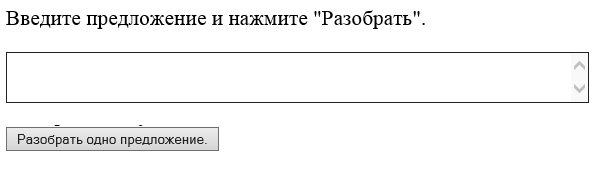
\includegraphics[scale=1.0]{images/form.png}
	\caption{\small Форма ввода системы topor-web}
	\label{fig:form}
\end{figure} 

Введите предложение в текстовое поле и нажмите кнопку <<Разобрать>>.
Пример разбора показан на рисунке \ref{fig:parse}.

\begin{figure}[H]
	\centering
		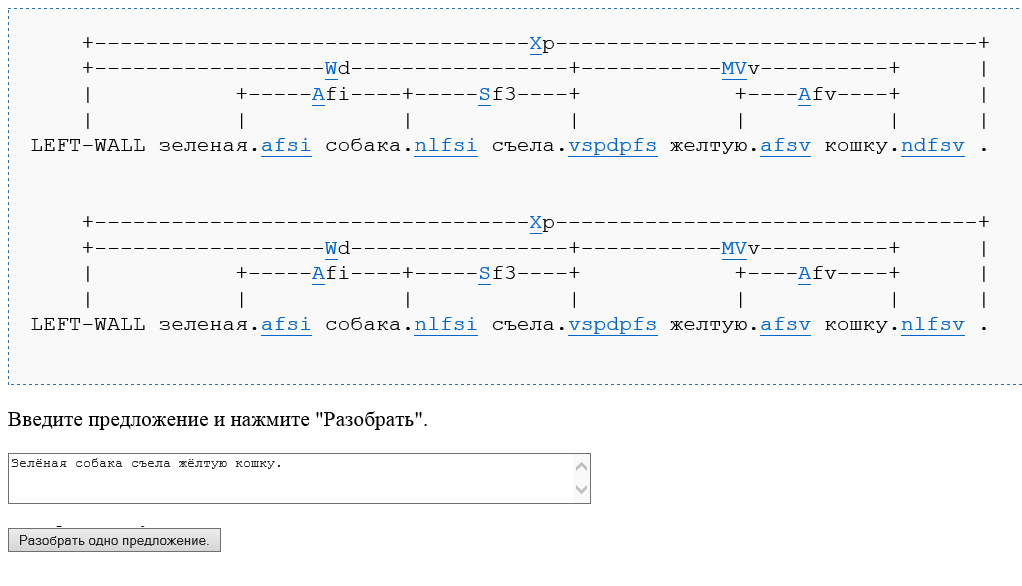
\includegraphics[scale=0.5]{images/parse.png}
	\caption{\small Пример разбора}
	\label{fig:parse}
\end{figure} 

Структура, представленная над полем ввода на рисунке \ref{fig:parse} является
деревом синтаксического разбора. Синий подчёркнутый текст – применяемые
к элементам предложения правила из онтологии.

\subsection{Результаты и выводы по главе 4}

В процессе работы над главой 4 были достигнуты следующие результаты:
\begin{list}{\labelitemi}{\leftmargin=1.5cm}
	\item рассмотрены детали инженерной реализации модуля взаимодействия парсера и онтологий tomahawk;
	\item составлено руководство по установке, настройки и работе с демонстрационной версией технологии topor-web.
\end{list}

\textbf{Вывод}: инженерная реализация спроектированного модуля выполнена успешно, полученной в процессе реализации информации достаточно для проведения экономического обоснования целесообразности внедрения предлагаемого решения.\newpage
  \indent \section{Экономическая эффективность применения модуля взаимодействия парсера русского языка с внешними онтологиями}

\subsection{Методы определения рыночной стоимости программного продукта}

Стоимость нематериальных активов зависит от способа их приобретения. Нематериальные активы могут быть внесены в качестве вклада в уставный капитал, приобретены за плату у других организаций, получены безвозмездно или созданы на самом предприятии. Поэтому оценка может быть произведена по договоренности сторон, исходя из затрат на приобретение, по рыночной стоимости, по стоимости изготовления.

Первоначальная стоимость нематериальных активов, внесенных в счет вклада в уставный капитал организации, определяется исходя из их денежной оценки, согласованной учредителями (участниками) организации, если иное не предусмотрено законодательством РФ.

Первоначальная стоимость нематериальных активов, приобретенных за плату, определяется как сумма всех фактических расходов на приобретение (за исключением налогов на добавленную стоимость и иных возмещаемых налогов) и приведение их в состояние, пригодное для использования в запланированных целях. 

Первоначальная стоимость нематериальных активов, полученных организацией по договору дарения (безвозмездно), соответствует их рыночной стоимости на дату принятия к бухгалтерскому учету.

Первоначальная стоимость нематериальных активов, созданных самой организацией, рассчитывается как сумма всех фактических расходов на их создание, изготовление (израсходованные материальные ресурсы, оплата труда, услуги сторонних организаций, патентные пошлины, связанные с получением патентов, свидетельств, и т.п.), за исключением налогов на добавленную стоимость и иных возмещаемых налогов.

Первоначальная стоимость нематериальных активов, полученных по договорам, предусматривающим исполнение обязательств (оплату) неденежными средствами, определяется исходя из стоимости товаров, переданных или подлежащих передаче организацией. Стоимость этих товаров устанавливают исходя из цены, по которой в сравнимых обстоятельствах обычно организация определяет стоимость аналогичных товаров.

Стоимость нематериальных активов, по которой они приняты к бухгалтерскому учету, не подлежит изменению, кроме случаев, установленных законодательством РФ.

Оценка нематериальных активов, стоимость которых при приобретении определена в иностранной валюте производится в рублях путем пересчета иностранной валюты по курсу Центрального банка РФ, действующему на дату приобретения организацией объектов по праву собственности, хозяйственного ведения, оперативного управления.

В оценке нематериальных активов можно использовать три основных подхода: доходный, затратный, сравнительный.

\subsection{Сравнительный подход}

Сравнительный подход используется при оценке рыночной стоимости нематериальных активов исходя из данных о недавно совершенных сделках с аналогичными нематериальными активами. 

Сравнительный подход может применяться для тех видов нематериальных активов, сделки по которым часто совершаются на рынке. Исходной информацией для расчета стоимости объекта служат цены продажи аналогичных объектов.

Метод базируется на принципе замещения, согласно которому рациональный инвестор не заплатит за данный объект больше, чем стоимость доступного к покупке аналогичного объекта, обладающего такой же полезностью, что и данный объект. Поэтому цены продажи аналогичных объектов служат исходной информацией для расчета стоимости данного объекта.

Расчеты методами, использующими сравнительный подход осуществляются по следующим этапам.

Этап 1. Изучение соответствующего рынка и сбор информации о недавних сделках с аналогичными объектами на данном рынке. Точность расчетов в значительной мере зависит от количества и качества собранной информации. Когда информации достаточно, необходимо убедиться, что проданные объекты действительно сопоставимы с оцениваемыми нематериальными активами по своим функциям и параметрам.

Этап 2. Проверка информации. Необходимо убедиться, прежде всего в том, что цены не искажены какими-либо чрезвычайными обстоятельствами, сопутствовавшими состоявшимся сделкам. Проверяется также достоверность информации о дате сделки, физических и других характеристиках аналогичных объектов.

Этап 3. Сравнение оцениваемого объекта с каждым из аналогичных объектов и выявление отличия по дате продажи, потребительским характеристикам, местоположению, исполнению, наличию дополнительных элементов и т.д. Все различия должны быть зафиксированы и учтены.

Этап 4. Расчет стоимости данных нематериальных активов путем корректировки цен на аналогичные нематериальные активы. В той мере, в какой оцениваемый объект отличается от аналогичного, в цену последнего вносят поправки с тем, чтобы определить, по какой цене мог быть продан объект, если бы обладал теми же характеристиками, что и оцениваемый объект. При анализе цен аналогичных объектов могут применяться следующие расчетные процедуры:

\begin{list}{\labelitemi}{\leftmargin=1.5cm}
	\item определение стоимости дополнительных элементов путем парных сравнений;
	\item определение корректирующих коэффициентов, учитывающих различия между объектами по отдельным параметрам;
	\item расчет стоимости по удельным стоимостным показателям, единым для определения группы аналогичных объектов;
	\item расчет стоимости с помощью мультипликатора дохода;
	\item расчет стоимости с помощью корреляционных моделей.
\end{list}

Определение стоимости дополнительных элементов осуществляется путем сравнения цен у двух групп объектов: имеющих и не имеющих эти элементы. Например, таким образом можно определить стоимость вспомогательных устройств к станкам, вспомогательных сооружений к зданиям и т.п.

Определение корректирующих коэффициентов используется тогда, когда сравниваемые нематериальные активы различаются по отдельным техническим и размерным параметрам. Качество и уровень функционирования, комфортности, удобства обслуживания --- все эти характеристики можно учесть в стоимости введения соответствующих повышающих или понижающих коэффициентов.

Расчет стоимости по удельным показателям --- способ, применяемый в тех случаях, когда сравниваемые объекты функционально однородны, но существенно различаются по размеру и мощности. При этом выводятся удельные цены на выбранную единицу. 

Способ расчета стоимости с помощью мультипликатора дохода, представляющего собой отношения цены аналогичного объекта к ежегодному доходу его владельца; применим к тем нематериальным активам, функционирование которых приносит доход. Если оценивают нематериальные активы предприятия в целом, то применяют мультипликатор Р/Е (цена к доходу на акцию), если оценивают нематериальные активы, включающие только недвижимость предприятия, то расчет ведут с помощью мультипликатора валового рентного дохода GRM, который представляет собой отношение цены аналогичного объекта к валовой ренте его владельца. Порядок расчета такой. Для каждого аналогичного объекта рассчитывают мультипликатор дохода, затем выводят усредненное значение мультипликатора для всей группы объектов. Стоимость данного объекта получают умножением усредненного мультипликатора на прогнозируемую величину дохода от данного объекта.

Расчет стоимости нематериальных активов с помощью корреляционной модели возможен в том случае, когда имеется достаточно большое количество аналогичных объектов и можно путем статистической обработки информации построить корреляционную модель, описывающую зависимость вероятной цены объекта от 2-3 его основных параметров.

С помощью описанного подхода оценим стоимость предлагаемого решения. В качестве аналогов приведём наиболее заметные программные реализации методов, приведённых в главе 1 и прототип --- Link Grammar Parser (таблица \ref{tab:anal}). Поскольку выбранные аналоги значительно отличаются друг от друга в объёмах реализованных функций, в то время как принципиально их функции однородны, выберем метод сравнения по удельным показателям. В качестве единицы сравнения примем стоимость одного года эксплуатации (затраты на поддержку решения в случае его исходной бесплатности и т. п.).

\begin{table}[H]
\centering
\caption{Рыночная стоимость аналогов}
{\small 
\begin{tabu}to \textwidth{ | X[c] | X[c] | }
	\hline
    Аналог      & Удельная стоимость года эксплуатаци, тыс. рублей  \\ \hline
	Oracle Text (часть Oracle Database EE, реализует методы CYK и алгоритм Эрли)   & 220 \\ \hline
	ABBYY Compreno (иерархические семантики, грамматики связей) & 100 \\ \hline
	SOLARIX (контекстно-независимые грамматики, метод Эрли) & 59 \\ \hline
	DictaScope (контекстно-независимые грамматики в НФХ) & 75 \\ \hline
	Link Grammar Parser (грамматика связей)    & 120 \\ \hline
	Среднерыночное значение & 114.8 \\ \hline
\end{tabu}
}
\label{tab:anal}
\end{table} 

В таблице \ref{tab:anal2} приведены результаты сравнения рыночных стоимостей  предлагаемого решения и прототипа, рассчитанные по методу прямого анализа продаж. Из таблицы видно, что предлагаемое решение экономически более эффективно, чем прототип.

\begin{table}[H]
\centering
\caption{Сравнение рыночной стоимости прототипа и предлагаемого решения}
{\small 
\begin{tabu}to \textwidth{ | X[c] | X[c] | X[c] | }
	\hline
    Критерий      & Предлагаемое решение & Прототип  \\ \hline
    Рыночная стоимость, тыс. рублей & 114.8 & 120 \\ \hline
\end{tabu}
}
\label{tab:anal2}
\end{table} 

\subsection{Затратный подход}

На основе затратного подхода определяют стоимость воспроизводства. Хотя при затратном подходе оцененная стоимость может значительно отличаться от рыночной стоимости, так как между затратами и полезностью нет прямой связи, тем не менее встречается немало случаев, когда оправдан именно затратный подход (например, для исчисления налога на имущество, для целей страхования отдельных составляющих имущества, при судебном разделе имущества между собственниками, при распродаже имущества на открытых торгах, для бухгалтерского учета основных фондов, при переоценке основных фондов).

В условиях России, где фондовый рынок только формируется, и рыночная информация почти отсутствует, затратный подход часто оказывается единственно возможным. 

Главный признак затратного подхода --- это поэлементная оценка, то есть оцениваемые нематериальные активы расчленяются на составные части, делается оценка каждой части, а затем стоимость всех нематериальных активов получают суммированием стоимостей его частей. При этом исходят из того, что у инвестора в принципе есть возможность не только купить данные нематериальные активы, но и создать их из отдельно покупаемых элементов.  

В зависимости от характера оцениваемых нематериальных активов применяют различные методы затратного подхода. Поэтому здесь речь идет об общей последовательности расчетов по данному подходу, выполняемых в несколько этапов. 

Этап 1. Анализ структуры нематериальных активов и выделение их составных частей (компонентов), оценка стоимости которых будет производиться дифференцированно различными методами. Если нужно оценить предприятие в целом, а не только его нематериальные активы, то в нем выделяют такие компоненты как: основные фонды (земля, здания, сооружения, машины и оборудование), оборотные материальные средства, денежные средства. 

Этап 2. Выбор наиболее походящего метода оценки стоимости для каждого компонента нематериальных активов и выполнение расчётов. Для определения стоимости земельного участка применяют специальные методы, известные из теории оценки недвижимости, или расчёты ведут по ценам за 1 $м^2$, применяемым при исчислении земельного налога. 

Этап 3. Оценка реальной степени износа компонентов нематериальных активов. Термин <<износ>> в теории оценки понимается как утрата полезности объекта, а следовательно и его стоимости по различным причинам, то есть не только вследствие фактора времени. Этот термин в ином смысле употребляется в бухгалтерском учете, где под износом или амортизацией понимается механизм переноса издержек на себестоимость продукции на протяжении нормативного срока службы объекта. 

В практике оценки различают два вида износа: физический износ и моральный износ. Физический износ означает потерю физических возможностей объекта в процессе его эксплуатации. Оценка морального износа в значительно большей степени пригодна в отношении ПП. Моральный износ характеризует потерю конкурентоспособности и соответственно стоимости, в связи с появлением на рынке новых более совершенных аналогов. Моральный износ принято подразделять на технологический, функциональный и внешний.

Технологический износ является следствием влияния на стоимость достижений научно-технического прогресса в области конструкции, технологии, материалов. 

Функциональный износ есть следствие уменьшения функциональных возможностей оцениваемого объекта в сравнении с новым аналогом. 

Внешний износ проявляется в том, что объект в какой-то момент перестает отвечать новым требованиям и ограничениям, например, по экологическим причинам, безопасности и т.д. 

Основным методом определения морального износа является метод сравнения с новым, более совершенным объектом. 

Этап 4. Расчет остаточной стоимости компонентов нематериальных активов и суммарная оценка остаточной стоимости всех нематериальных активов. Остаточная стоимость на дату оценки получается вычитанием из стоимости размера накопленного износа. 

Применительно к таким объектам, как ноу-хау и изобретения, аннуитетом служат платежи роялти, то есть ежегодно выплачиваемые предприятием-лицензиатом суммы обладателю ноу-хау или патента (лицензиару), согласно заключенному между ними договору. 

Оценим стоимость предлагаемого решения на основе описанного подхода. Для учёта износа объекта оценки рассчитаем норму амортизации по формуле (4).

\begin{equation}
	K = (1 / N) \cdot 100\% 
\end{equation}

K --- норма амортизации, N --- срок полезного использования (в месяцах). Принимая срок полезного использования ПП в 5 лет, получаем норму амортизации равной 1.67\%.

Для расчёта ежемесячной суммы амортизации используется формула (5).

\begin{equation}
	A = (K / 100\%) \cdot S
\end{equation}

A --- ежемесечная сумма амортизации, K --- норма амортизации, S --- стоимость объекта, рассчитанная методом восстановленной стоимости.

Для расчёта восстановленной стоимости предлагаемого решения просуммируем затраты на его создание (таблица \ref{tab:cost}).

\begin{table}[H]
\centering
\caption{Затраты на создание предлагаемого решения}
{\small 
\begin{tabu}to \textwidth{ | X[c] | X[c] | }
	\hline
	Тип & Значение (тыс. рублей) \\ \hline
	Заработная плата разработчику в течение всего срока разработки & 90 (30 x 3) \\ \hline
    Затраты на компьютерное оборудование & 40  \\ \hline
    Затраты на электроэнергию & 9 (3 x 3) \\ \hline
    Затраты на ПО разработки & 3 \\ \hline
    Амортизация в течение срока разработки & 7.11 (1.67 * 142 * 3 / 100) \\ \hline
    Итого & 149.11 \\ \hline
\end{tabu}
}
\label{tab:cost}
\end{table} 

Аналогично рассчитаем затраты на восстановление прототипа Link Grammar Parser, учитывая срок разработки в 3 месяца и отличные от РФ заработные платы разработчикам (таблица \ref{tab:cost1}).

\begin{table}[H]
\centering
\caption{Затраты на восстановление прототипа}
{\small 
\begin{tabu}to \textwidth{ | X[c] | X[c] | }
	\hline
	Тип & Значение (тыс. рублей) \\ \hline
	Заработная плата разработчику в течение всего срока разработки & 300 (100 x 3) \\ \hline
    Затраты на компьютерное оборудование & 120  \\ \hline
    Затраты на электроэнергию & 9 (3 x 3) \\ \hline
    Затраты на ПО разработки & 0 (использовалось открытое ПО) \\ \hline
    Амортизация в течение срока разработки & 21,49 (1.67 * 429 * 3 / 100) \\ \hline
    Итого & 450.49 \\ \hline
\end{tabu}
}
\label{tab:cost1}
\end{table} 

Сравним затраты на разработку предлагаемого решения и на восстановление прототипа (таблица \ref{tab:costs}).

\begin{table}[H]
\centering
\caption{Сравнение затрат на создание предлагаемого решения и восстановление прототипа}
{\small 
\begin{tabu}to \textwidth{ | X[c] | X[c] | X[c] |}
	\hline
	Критерий & Предлагаемое решение & Прототип \\ \hline
	Стоимость разработки (тыс. рублей) & 149.11 & 450.49 \\ \hline
\end{tabu}
}
\label{tab:costs}
\end{table} 

Таким образом, по результатам оценки с использованием затратного подхода, разработка предлагаемого решения является целесообразной.


\newpage
  \indent \section{Заключение}\newpage
  \renewcommand*{\refname}{}
\section*{\centering СПИСОК ИСПОЛЬЗОВАННЫХ ИСТОЧНИКОВ}
\addcontentsline{toc}{section}{СПИСОК ИСПОЛЬЗОВАННЫХ ИСТОЧНИКОВ}
\begin{thebibliography}{99}	
	\bibitem{academica_nl}
	Словарь социолингвистических терминов. Академика. [Электронный ресурс] --- Режим доступа: \url{http://sociolinguistics.academic.ru/185}. Дата обращения 21.05.2013.

	\bibitem{wiki_nlp}
	Natural language processing [Электронный ресурс] --- Режим доступа: \url{http://en.wikipedia.org/wiki/Natural_language_processing}. Дата обращения 20.05.2013.	

	\bibitem{wiki_parsing}
	Parsing [Электронный ресурс] --- Режим доступа: \url{http://en.wikipedia.org/wiki/Parsing}. Дата обращения 21.05.2013.	

	\bibitem{wiki_fg}
	Formal grammar [Электронный ресурс] --- Режим доступа: \url{https://en.wikipedia.org/wiki/Formal_grammar}. Дата обращения 21.05.2013.

	\bibitem{academica_loc}
	Финансовый словарь. Академика. [Электронный ресурс] --- Режим доступа: \url{http://dic.academic.ru/dic.nsf/fin_enc/24769}. Дата обращения 21.05.2013.

	\bibitem{samuel}
	Samuel A. L. Some Studies in Machine Learning Using the Game of Checkers. // IBM Journal. 1959.	

	\bibitem{wiki_semantic_web} 
	Semantic Web [Электронный ресурс] --- Режим доступа: \url{http://en.wikipedia.org/wiki/Semantic_Web}. Дата обращения 20.05.2013.	

	\bibitem{wiki_rdf}
	Resource description framework [Электронный ресурс] --- Режим доступа: \url{http://ru.wikipedia.org/wiki/Resource_Description_Framework}. Дата обращения 21.05.2013.	

	\bibitem{wiki_ont}
	Ontology [Электронный ресурс] --- Режим доступа: \url{http://en.wikipedia.org/wiki/Ontology_(information_science)}. Дата обращения 21.05.2013. 

	\bibitem{google}
	Google Search [Электронный ресурс] --- Режим доступа: \url{http://google.com}. Дата обращения 20.05.2013.

	\bibitem{bing}
	Microsoft Bing [Электронный ресурс] --- Режим доступа: \url{http://bing.com}. Дата обращения 20.05.2013.

	\bibitem{yandex}
	Yandex [Электронный ресурс] --- Режим доступа: \url{http://ya.ru}. Дата обращения 20.05.2013.

	\bibitem{tsaati}
	Саати, Т. Принятие решений. Метод анализа иерархий. Издательство: М.: Радио и связь. 1993.	

	\bibitem{eisner}
	Eisner J.M. Three New Probabilistic Models for Dependency Parsing: An Exploration. // Proceedings of the 16th International Conference on Computational Linguistics. – 1996.

	\bibitem{wiki_cyk}
	CYK algorithm [Электронный ресурс] --- Режим доступа: \url{http://en.wikipedia.org/wiki/CYK_algorithm}. Дата обращения 28.05.2013.	

	\bibitem{webbe}
	Webbe B. Chart Parsing: The Earley Algorithm. --- 2007.

	\bibitem{sleator}
	Sleator D.D.K. Parsing English with a Link Grammar. --- 1991.

	\bibitem{wiki_modelling}
	Моделирование [Электронный ресурс] --- Режим доступа: \url{http://ru.wikipedia.org/wiki/Моделирование}. Дата обращения 30.05.2013.

	\bibitem{uemov}
	Уёмов А. И. Логические основы метода моделирования, М.: Мысль, 1971.

	\bibitem{gold}
	Гольдштейн С.Л., Ткаченко Т.Я. Введение в системологию и системотехнику.

	\bibitem{abiparser}
	Link Grammar Parser [Электронный ресурс] --- Режим доступа: \url{http://www.abisource.com/projects/link-grammar/}. Дата обращения: 03.06.2013.	

	\bibitem{api}
	The Link Parser API [Электронный ресурс] --- Режим доступа: \url{http://www.abisource.com/projects/link-grammar/api/index.html}. Дата обращения 03.06.2013.	

	\bibitem{gpl}
	Стандартная общественная лицензия GNU [Электронный ресурс] --- Режим доступа: \url{http://www.gnu.org/licenses/gpl.html}. Дата обращения: 03.06.2013.

	\bibitem{haskell}
	The Haskell Programming Language [Электронный ресурс] --- Режим доступа: \url{http://www.haskell.org/haskellwiki/Haskell}. Дата обращения: 03.06.2013.

	\bibitem{haskell2010}
	Announcing Haskell 2010 [Электронный ресурс] --- Режим доступа: \url{http://www.haskell.org/pipermail/haskell/2009-November/021750.html}. Дата обращения: 04.06.2013.
\end{thebibliography}\newpage
  \indent \section{Приложение А. Техническое задание на разработку модуля взаимодействия парсера русского языка с онтологиями}
\end{document}
